\chapter{自适应噪声矫正调制识别网络}\label{chap:intro}
\markboth{第三章\ \ 自适应噪声矫正调制识别网络}{}
% 第三章“自适应噪声矫正调制识别网络”的撰写思路可以分为以下几个关键部分:

% 1. **引言和背景介绍**
%    - 简要回顾第一章和第二章的内容,尤其是关于数字调制信号模型和深度学习理论基础的部分。
%    - 强调噪声对调制识别准确性的影响,以及解决这一问题的重要性。
%    - 介绍目前解决噪声问题的主流方法,以及它们的局限性。

% 2. **自适应噪声矫正模块的设计和原理**
%    - 详细描述自适应噪声矫正模块的设计思路和工作原理。
%    - 使用数学公式和图表来解释噪声矫正的机制。
%    - 讨论该模块如何根据信号的噪声水平动态调整其矫正策略。

% 3. **特征提取模块的改进**
%    - 介绍传统特征提取方法及其不足。
%    - 详细阐述通过改进软阈值化技术所提出的特征提取模块。
%    - 讨论如何通过该模块更有效地提取调制信号的特征。

% 4. **网络结构和实现**
%    - 描述整个调制识别网络的架构,包括自适应噪声矫正模块和特征提取模块在内的各个组件。
%    - 讨论网络的实现细节,包括层的类型、激活函数的选择等。

% 5. **实验结果和分析**
%    - 展示在不同信噪比条件下的实验结果,包括与传统方法的比较。
%    - 分析自适应噪声矫正模块和改进的特征提取模块对性能提升的贡献。
%    - 讨论实验结果的意义,以及该方法在实际应用中的潜力。

% 6. **小结**
%    - 总结本章的主要内容和创新点。
%    - 简要讨论本章工作对未来研究的影响和可能的发展方向。

% 通过上述撰写思路,第三章将系统地展示自适应噪声矫正调制识别网络的设计、实现及其效果,明确地展示该方法在调制识别领域的创新性和实用性。

\section{引言与相关背景}\label{sec:background}

% 随着通信环境的不断复杂化,自动调制识别性能逐渐成为实际应用中备受关注的焦点。该性能受到多种实际环境因素的复合影响,其中包括噪声、多径效应和多普勒效应等。噪声由于其在实际环境中的变化性和强度的不断波动,因而成为主要的制约因素之一。

% 为迎接这一挑战,自动调制识别系统急需在各种噪声环境下保持一定的鲁棒性,以确保有效完成自动调制识别任务。为实现这一目标,本研究提出了一种自适应降噪的自动调制识别网络(Adaptive Denoising Automatic Modulation Recognition Network,AD-AMR Net)。

% 该网络由两个关键组成部分构成,即自适应降噪模块和特征提取模块,并在这两个模块中引入了高效通道注意力模块以进一步优化性能。自适应降噪模块通过对噪声分布的自适应学习,实现对输入信号的降噪,从而提高整个自动调制识别系统的鲁棒性。另一方面,特征提取模块引入了改进的软阈值化模块,以提取更为具体的特征,从而提升系统的识别准确性。

% 通过详实的实验验证,本研究充分证明了提出的自适应降噪自动调制识别网络在实际应用中的显著有效性,为在复杂噪声环境下更精准地区分不同调制模式提供了有力的支持。本章首先介绍了高效通道注意力模块(Efficient Channel Attention,ECA)的原理,随后详细阐述了自适应降噪自动调制识别网络的设计思路和实现方法,分别介绍了自适应降噪模块(Adaptive Denoising Module,ADM)和特征提取模块(Feature Extraction Module,FEM)。接着,对该网络的性能进行了充分的实验验证,最终对本章进行了总结。具体框架如图\ref{fig:ad-amr-overview}所示。

\begin{figure}
    \centering
    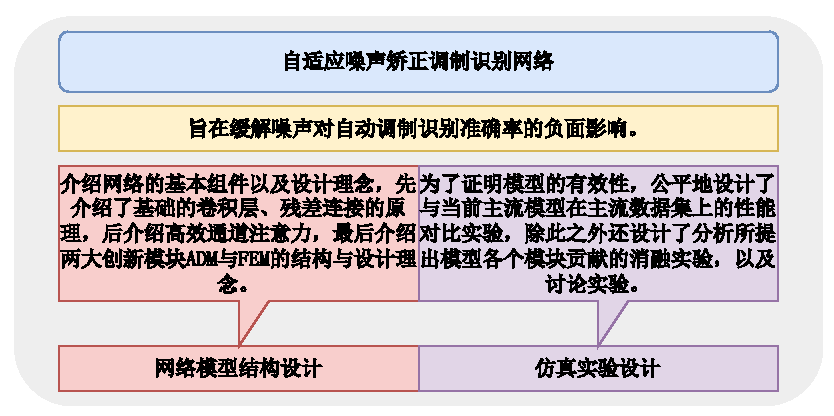
\includegraphics[width=0.9\textwidth]{Image/chap3_map.pdf}
    \caption{本章大纲}
    \label{fig:ad-amr-overview}
\end{figure}

随着通信环境变得日益复杂,自动调制识别(Automatic Modulation Recognition, AMR)系统的性能受到了极大的关注。在实际应用场景中,AMR系统的表现受到诸多环境因素的影响,其中包括噪声、多径效应、多普勒效应等。特别是噪声,由于其不可预测性和变化性,尤其是在现实环境中的强度波动,成为了影响AMR系统性能的主要挑战。

为了应对这一挑战,我们认识到在各种噪声环境下,AMR系统需要具备更强的鲁棒性,以确保其有效性和可靠性。基于此,本研究提出了一种创新的自适应噪声矫正自动调制识别网络(Adaptive Denoising Automatic Modulation Recognition Network, AD-AMR Net),旨在提高系统在不同噪声条件下的调制识别精度和鲁棒性。AD-AMR Net主要由两个核心组成部分构成:自适应噪声矫正模块(Adaptive Denoising Module, ADM)和特征提取模块(Feature Extraction Module, FEM)。在这两个模块中,我们均采用了高效通道注意力模块(Efficient Channel Attention, ECA),以进一步提升网络性能。ADM致力于对噪声分布进行自适应学习,以有效降低输入信号的噪声,从而增强整个AMR系统的鲁棒性。与此同时,特征提取模块利用改进的软阈值化策略,高效提取信号的关键特征,进而提升系统的识别精度。

在实验设计方面,我们精心安排了一系列对比实验,在公开数据集上将AD-AMR Net与近年来的主流模型进行了公平比较。这些实验旨在突出AD-AMR Net在性能方面的优势。此外,为了深入了解网络内各模块的具体作用,我们设计了消融实验。通过这些实验,我们不仅能够评估各个模块对整体性能的贡献,还能探究AD-AMR Net在不同模块组合下的表现。最后,我们还讨论了ADM模块的即插即用特性,即将其集成到其他主流网络中后对性能的提升效果。这些实验结果为评估AD-AMR Net的有效性和灵活性提供了重要依据。



\section{网络模型结构设计}\label{sec:background}

\subsection{卷积层}\label{sec:background}

在深度学习中,卷积层的应用极为广泛,尤其是在图像处理和时间序列数据分析领域。为了全面理解卷积层的工作原理和其强大的功能,本章节将深入探讨卷积层的特点、计算公式以及应用场景。

卷积层通过其独特的参数共享和局部连接机制实现了高效的特征提取。参数共享意味着相同的卷积核在整个输入数据上滑动,从而显著减少了模型的参数数量。而局部连接则确保卷积层能够捕捉到输入数据的局部特征。此外,卷积层由于其设计特性,具有一定程度的平移不变性,使得它能够在不同位置识别相同的特征。卷积层的基本操作可以用以下数学公式表达:
\begin{align}
    \text{Output}(i, j) = \sum_{m}\sum_{n} \text{Kernel}(m, n) \times \text{Input}(i-m, j-n),
    \label{equ: conv}
\end{align}
此公式中,Output表示输出的特征图,Kernel是卷积核,Input是输入的特征图,而m和n代表卷积核在输入上的位置。

\begin{figure}
    \centering
    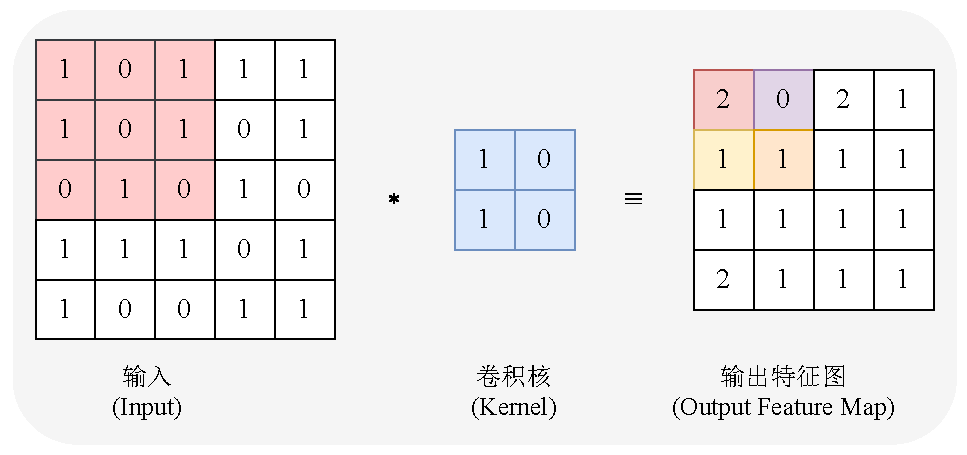
\includegraphics[width=\textwidth]{Image/conv.pdf}
    \caption{卷积操作示意图}
    \label{fig:conv}
\end{figure}

为了更直观地展示卷积操作,图\ref{fig:conv}呈现了一个简化的二维卷积过程。如图所示,输入数据(Input Data)是一个较大的二维网格,卷积核(Convolution Kernel)在其上滑动并执行卷积操作,产生输出特征图(Output Feature Map)。这种视觉表示有助于理解卷积层如何在局部区域应用卷积核来提取特征。


在应用方面,卷积层根据处理数据的维度和特性分为不同的类型。二维卷积(2D Convolution)主要用于处理图像等二维数据,其卷积核在输入图像的高度和宽度两个维度上移动,非常适合提取空间特征。而一维卷积(1D Convolution)则更适用于处理如音频信号或某些金融时间序列这类的一维数据,其卷积核仅沿一个维度(通常是时间轴)移动,有效地捕获序列数据中的时间特征。其数学公式如下:

\begin{align}
    \text{Output}(i) = \sum_{m} \text{Kernel}(m) \times \text{Input}(i-m),
    \label{equ: onedconv}
\end{align}

综上所述,卷积层在现代深度学习架构中扮演着至关重要的角色。它们不仅在图像处理领域展现出强大的能力,也在时间序列数据分析中显示出巨大的潜力,提供了一种强大的方法来提取和分析数据中的关键特征。

\subsection{残差连接}\label{sec:background}

\begin{figure}
    \centering
    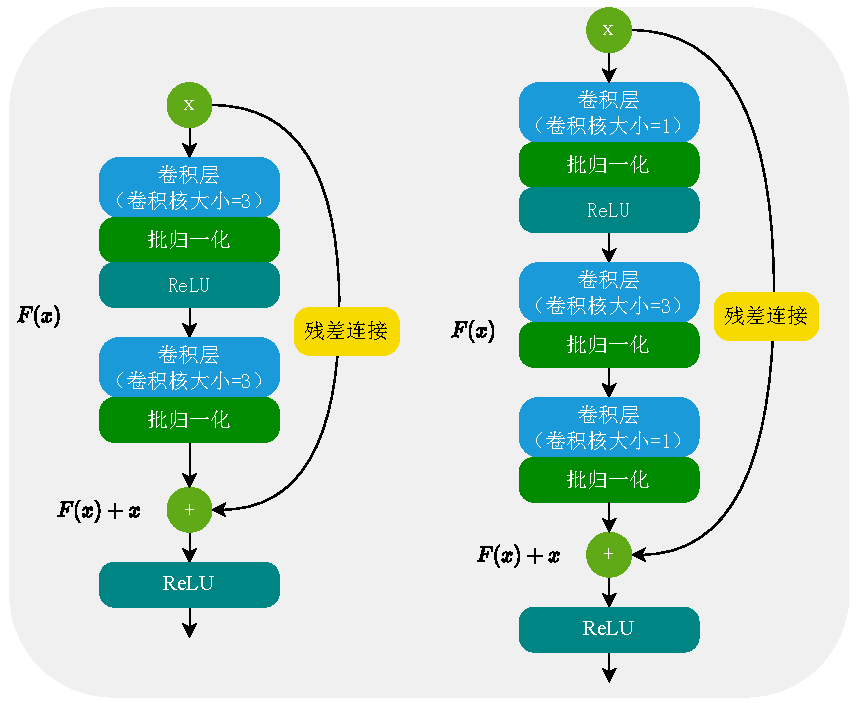
\includegraphics[width=0.8\textwidth]{Image/residualblock_cn.pdf}
    \caption{残差连接示意图,其中左边为普通残差块,右边为瓶颈残差块}
    \label{fig:residual}
\end{figure}

在深度学习的发展过程中,随着神经网络结构变得越来越深,网络的训练变得日益困难。这主要是因为在深层网络中常见的梯度消失和梯度爆炸问题,这些问题严重影响了网络性能的提升和模型的训练效率。为了克服这些挑战,残差连接(Residual Connection)的概念被引入到深度神经网络的设计中\cite{he2016deep},特别是在复杂的图像处理任务中。本章节旨在探讨残差连接的原理、其带来的实际效果,以及在实际应用中的重要性。

残差连接的核心思想是通过添加一种直接的路径,将输入信息直接传递到网络的后续层,从而解决深层网络中的信息流失问题。数学上,这可以表示为:

% \[ \text{Output} = \text{Activation}(\text{Conv}(X) + X) \]
\begin{align}
    \text{Output} = \text{Activation}(\text{Conv}(X) + X),
    \label{equ: residual}
\end{align}

在这个公式中,X代表输入特征图,Conv代表卷积层操作,Activation是激活函数,Output是残差块的输出。残差连接通过加法操作将输入直接与卷积层的输出相加,这种设计使得网络可以学习到输入与输出之间的残差,即输出与输入的差异。

残差连接的引入为深度学习带来了革命性的影响。在ResNet(Residual Network)等基于残差连接的架构中,网络能够通过残差连接维持较深层次时信息的流动性和有效性,从而避免了梯度消失的问题。实际效果中,ResNet架构在各种图像识别竞赛中取得了显著的成绩,比如在ImageNet挑战中大幅提升了分类精度,显示出强大的学习能力和泛化性能。

此外,残差连接的设计也促进了深层网络训练的稳定性。由于残差连接的存在,深层网络中的梯度能够有效地传递,大大减少了训练深层网络时的困难。这种优势使得研究人员能够构建更深层次的网络,探索更复杂的模型结构,从而在诸如图像分类、物体检测和语义分割等任务中取得更好的性能。

综合来看,残差连接不仅解决了深层网络训练中的关键难题,还推动了深度学习在诸多领域的广泛应用和快速发展。通过提供一种有效的信息传递机制,残差连接改善了深层神经网络的训练效果和模型性能,被视为现代深度学习架构设计中的一个重要里程碑。

% \subsection{高效通道注意力}\label{sec:background}
% \begin{figure}
%     \centering
%     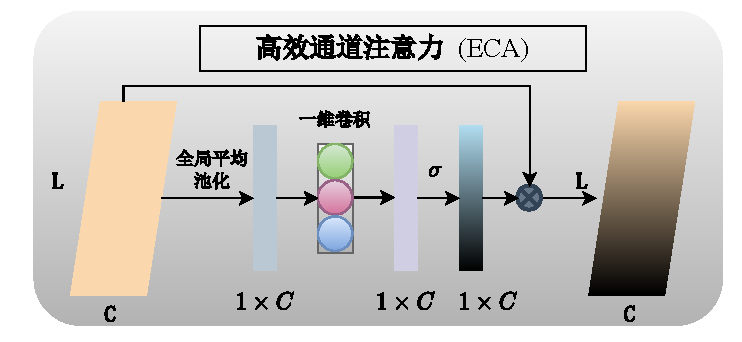
\includegraphics[width=0.6\textwidth]{Image/eca.jpg}
%     \caption{高效通道注意力模块}
%     \label{fig:eca}
% \end{figure}

% 通道注意机制(Channel Attention Mechanism, CAM)在当前的卷积神经网络中被广泛应用于各种任务。其中,挤压激励模块(Squeeze and Excitation Module, SEM)是一种备受欢迎的通道注意机制,它通过挤压和激励操作来捕捉通道之间的依赖关系。然而,SEM的一个局限性在于它依赖于计算开销较大的全连接层,用于学习注意力权重。尤其在输出通道较大的情况下,SEM可能导致显著的计算成本,同时还会增加网络的内存占用,限制了其在资源受限环境中的应用。

% 为了解决这一问题,我们引入了ECA模块,这是一种轻量但高效的通道注意机制,专门设计用于实现高泛化能力。如图~\ref{fig:eca}所示,ECA模块由全局平均池化(Global Average Pooling, GAP)层、一维卷积层和sigmoid激活组成,因此需要的参数远远少于SEM。具体而言,GAP层将特征图总结成一个全局上下文向量,以捕捉跨通道的依赖关系。这种全局池化的思想受益于自然图像中的平移不变性,有助于捕捉特征的整体信息。

% 接着,一维卷积层将这个全局上下文向量转换为通道注意权重。相较于全连接层,卷积层具有参数共享和局部感受野的优势,使得ECA模块能够更加灵活地捕捉通道间的关系。通过sigmoid函数将注意权重缩放到0到1之间,sigmoid函数的定义如下:
% %sigmoid函数
% \begin{equation}
% \begin{aligned}
% \text{sigmoid}(x) = \frac{1}{1 + \text{exp}(-x)}.
% \end{aligned}
% \label{equ: sigmoid}
% \end{equation}

% 通过与输入特征进行逐元素乘法,ECA模块突出显示信息丰富的特征并抑制不太相关的特征。这种非线性的特征放大和抑制机制有助于提高模型对关键信息的关注度,从而提升性能。尽管ECA模块的设计相对简单,但经验结果表明,与SEM相比,它在使用更少的参数和计算资源的情况下能够实现更好的性能。这使得ECA模块成为计算通道注意力的一种高效且轻量级的选择。在实际应用中,ECA模块在图像分类、目标检测等任务中展现了出色的通用性和性能。

\subsection{高效通道注意力}\label{sec:background}
\begin{figure}
\centering
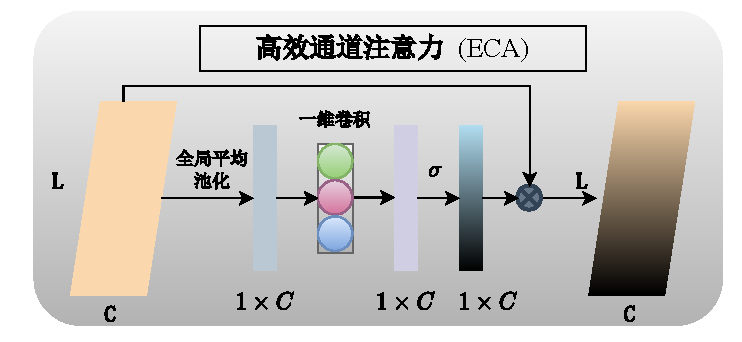
\includegraphics[width=0.8\textwidth]{Image/eca.pdf}
\caption{高效通道注意力模块}
\label{fig:eca}
\end{figure}

通道注意机制(Channel Attention Mechanism, CAM)已在现代卷积神经网络中被广泛应用于多种任务,以提升其性能。特别地\cite{wang2020eca},挤压激励模块(Squeeze and Excitation Module, SEM)是一种流行的CAM实现,它通过挤压和激励操作来有效捕获通道间的相关性。然而,挤压激励模块在学习注意力权重时依赖于计算成本较高的全连接层,特别是当输出通道数量较大时,可能带来显著的计算和内存开销,从而限制了其在资源有限的环境下的应用。

为应对这一挑战,我们引入了一种轻量级且高效的通道注意机制——高效通道注意力(ECA)模块。如图~\ref{fig:eca}所示,ECA模块是一种在现代卷积神经网络中应用的通道注意机制,它基于挤压和激励(squeeze-and-excitation, SE)模块的设计理念,但在减少模型复杂度方面做了改进,尤其是避免了维度降低的问题。ECA模块通过不进行通道维度的降低,能够更直接地捕捉不同通道间的关系,从而提高了注意力学习的效率。

具体来说,ECA模块首先利用全局平均池化(Global Average Pooling, GAP)操作来聚合特征,然后通过一维卷积来获取每个通道及其邻近通道的交互信息。这样的设计使得ECA模块可以更高效地实现局部跨通道的交互。此外,一维卷积的核大小(kernel size)决定了局部跨通道交互的覆盖范围,即决定了在注意力预测中有多少相邻通道参与。ECA模块的这种设计不仅降低了参数数量,而且提高了计算效率,使得它在大规模图像分类、目标检测等任务中表现出色。相较于传统的SE模块,ECA模块在资源受限的环境下具有更好的应用潜力。

在经过上述的运算之后ECA会得到一个$1 \times C$的权重向量,经过sigmoid函数处理,这些权重被缩放到0至1的范围内。sigmoid函数定义如下:
%sigmoid函数
\begin{equation}
\begin{aligned}
\text{sigmoid}(x) = \frac{1}{1 + \text{exp}(-x)}.
\end{aligned}
\label{equ: sigmoid}
\end{equation}

ECA模块通过与输入特征进行逐元素乘法操作,有效地突出显示重要特征并抑制不太相关的特征。这种非线性的特征增强和抑制机制显著提升了模型对关键信息的敏感度,进而提高整体性能。值得注意的是,尽管ECA模块的设计相对简单,但它在实际应用中——如图像分类、目标检测等任务——表现出了优异的通用性和性能,同时在参数和计算资源方面的经济性使其成为处理通道注意力的高效且轻量级的选择。

% \subsection{自适应噪声矫正模块具体设计}\label{sec:background}

% \begin{figure}
%     \centering
%     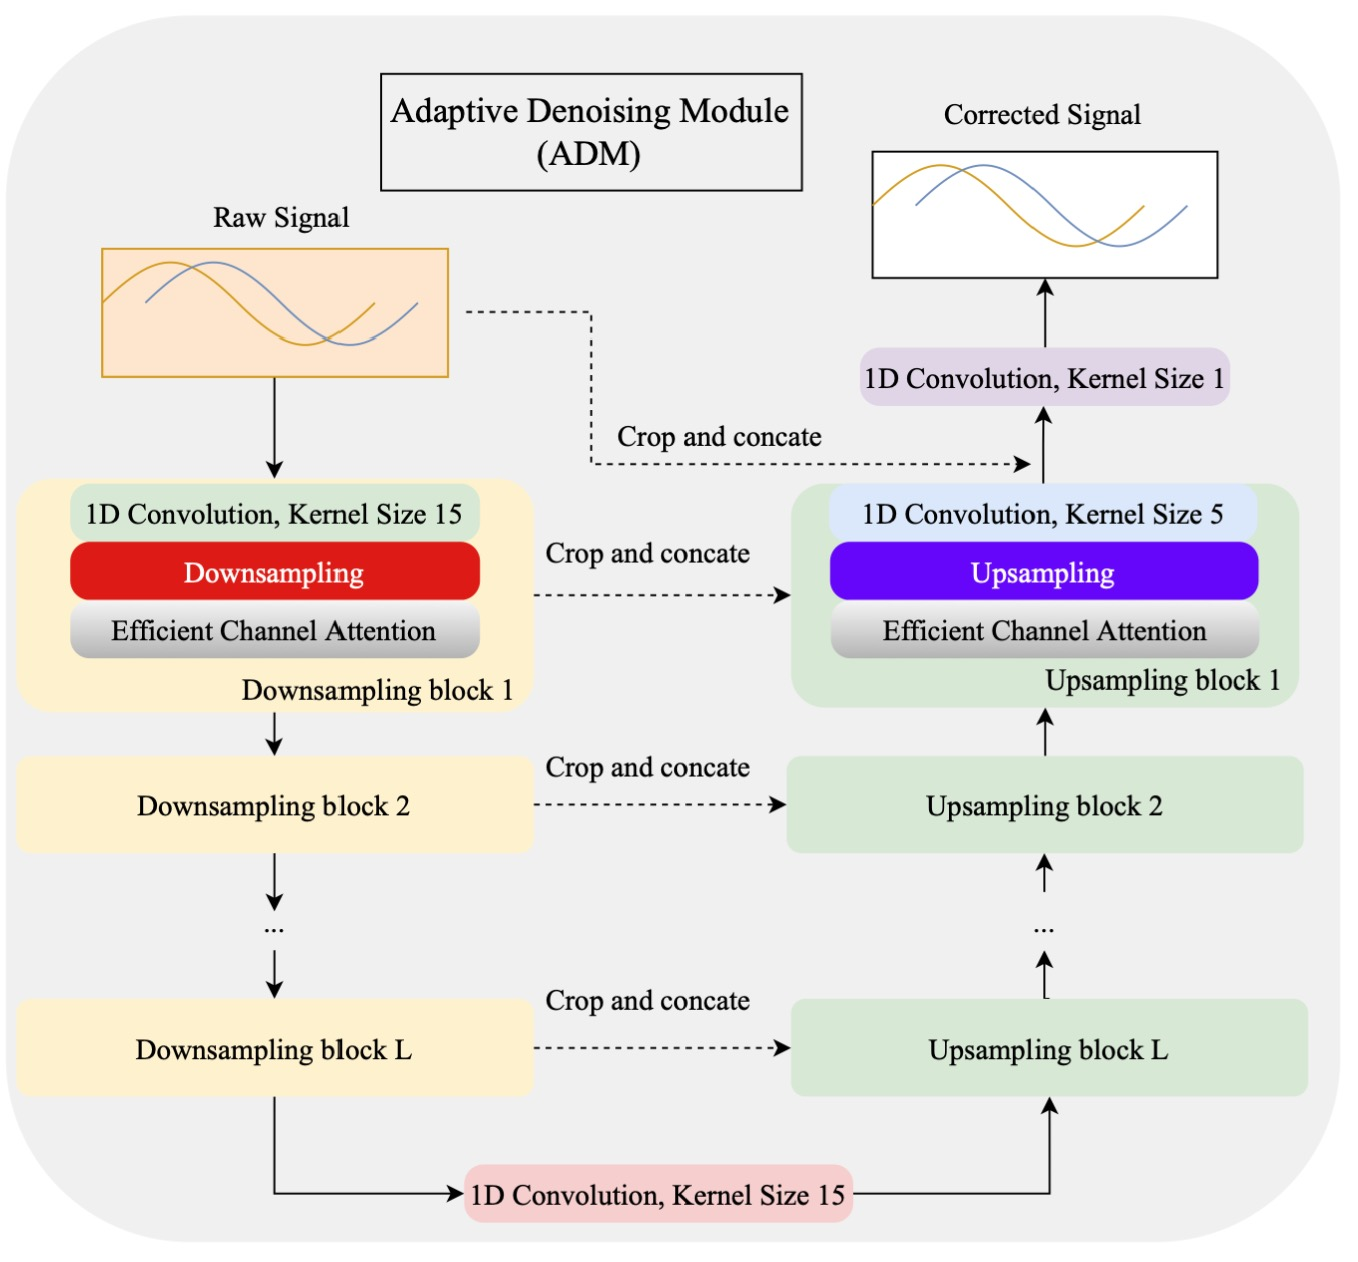
\includegraphics[width=0.6\textwidth]{Image/adm.jpg}
%     \caption{自适应降噪模块}
%     \label{fig:adm}
% \end{figure}

% 复杂信号作为一种时间序列数据,往往受到各种噪音和偏移的影响。在这种背景下,我们通过将ECA集成到WaveUNet架构中,提出了一种称为ADM(Adaptive Denoising Module)的解决方案,旨在有效减轻这些干扰的影响。ADM的设计灵感源自ECA和WaveUNet,结合了通道注意机制和波形处理网络的优势。

% ADM的核心目标是接收带有噪音的输入信号,并通过学习抑制噪音,同时保留信号的真实基础结构,从而生成一个去噪版本的输出。通过在网络的训练过程中,ADM部分成功地拟合了原始信号,使得输出信号更加清晰,噪音水平相应降低。这一观察结果得到了在文献中的验证~\cite{michelashvili2019speech}。

% ADM的架构如图~\ref{fig:adm}所示,包含了一系列下采样和上采样块。在这些块中,每个都包括一个1D卷积层(卷积核大小为15)用于学习局部特征,一个下采样或上采样操作以处理不同尺度的信息,以及一个ECA模块来强调具有信息量的特征。下采样的目的是在更广泛的上下文中整合信息,以及通过减少分辨率来关注大尺度信号组成部分,而上采样则恢复分辨率,并允许模型整合来自更粗糙尺度编码的信息。

% 关键的设计特点之一是通过裁剪和连接的跳跃连接,实现了编码信息在不同尺度之间的传递。这样的设计保留了本地和全局上下文,有助于捕捉信号的复杂结构。最终,通过一个1D卷积层(卷积核大小为1)在通道上整合,生成去噪输出。这个层级处理和聚合信息的过程使得ADM能够分离有意义的信号成分并抑制噪音,从而在实际应用中取得显著效果。

% 通过将嘈杂信号输入到ADM中,我们能够从中解开清晰信号的组成部分,从而在复杂信号处理中提供了一种有效的工具。这种整合了通道注意机制的ADM设计不仅在噪音抑制上取得了令人满意的效果,而且在保留信号关键特征的同时,减少了计算复杂度,使得其成为时间序列数据处理中的一种有前景的方法。

\subsection{自适应噪声矫正模块具体设计}\label{sec:background}

\begin{figure}
\centering
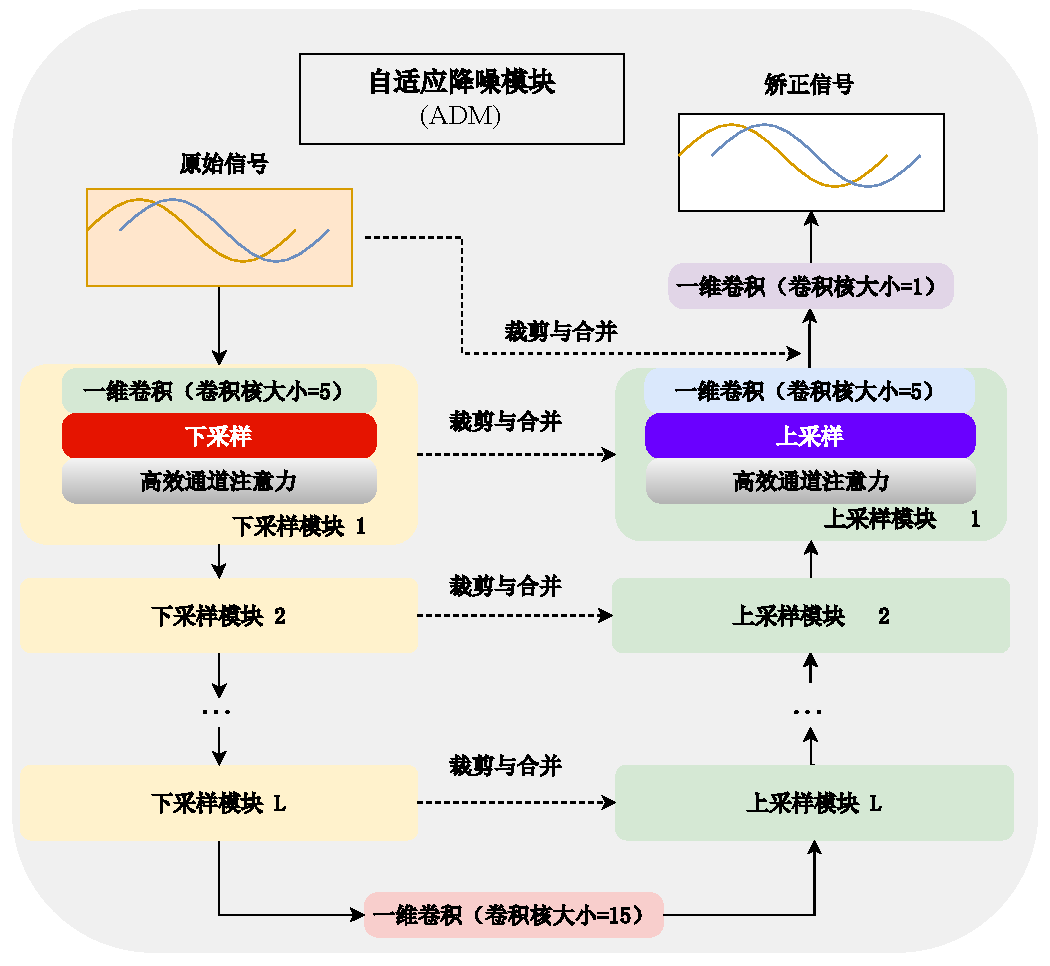
\includegraphics[width=0.8\textwidth]{Image/adm.pdf}
\caption{自适应降噪模块}
\label{fig:adm}
\end{figure}

在处理复杂的时间序列信号时,经常面临多种噪声和干扰的挑战。针对这一问题,我们结合了高效通道注意力(ECA)模块和WaveUNet架构的特性,设计了ADM(Adaptive Denoising Module)。ADM不仅从ECA中借鉴了通道注意机制的优势,还引入了WaveUNet在处理音频信号方面的深层次多尺度特征提取能力。

ADM的主要任务是接收带有噪声的输入信号,并通过先进的学习机制有效地降低噪声,同时保留信号的原始结构。其核心是利用WaveUNet的多层次结构来进行深入的信号分析。在训练过程中,ADM能够对原始信号进行高度拟合,从而在输出端提供更加清晰、噪声水平更低的信号。这一成果已得到相关研究的支持和验证~\cite{michelashvili2019speech}。

ADM的架构如图~\ref{fig:adm}所示,它包含了一系列的下采样和上采样块,类似于WaveUNet的设计。这些块中每个都包含一个1D卷积层(卷积核大小为15),用以学习局部特征,一个下采样或上采样操作处理不同尺度的信息,以及一个ECA模块以突出重要特征。下采样的目的是在更广泛的上下文中整合信息,并关注大尺度信号组成部分,而上采样则用于恢复分辨率,整合更粗糙尺度编码的信息。

特别地,ADM的一个关键设计特点是通过裁剪和连接实现的跳跃连接。这些连接在不同尺度之间传递编码信息,保留了局部和全局上下文,有助于捕捉信号的复杂结构。最终,一个1D卷积层(卷积核大小为1)在通道上进行整合,生成清晰的去噪输出。这种层级化的信息处理和聚合方式使得ADM不仅能够有效分离有意义的信号成分并抑制噪声,还能够在不增加过多计算负担的情况下,实现对信号细节的精确还原。

将含有噪声的信号输入ADM后,我们可以有效地提取出清晰的信号成分,尤其是在复杂的信号处理任务中,如音频信号分离、语音增强等应用场景。这种结合了通道注意力机制和多层次信号处理能力的ADM设计,不仅在噪声抑制方面表现出色,还在保持信号关键特征的同时优化了计算效率,展现出在复杂时间序列数据处理中的巨大潜力。

% \section{特征提取模块}\label{sec:background}

% \begin{figure}
%     \centering
%     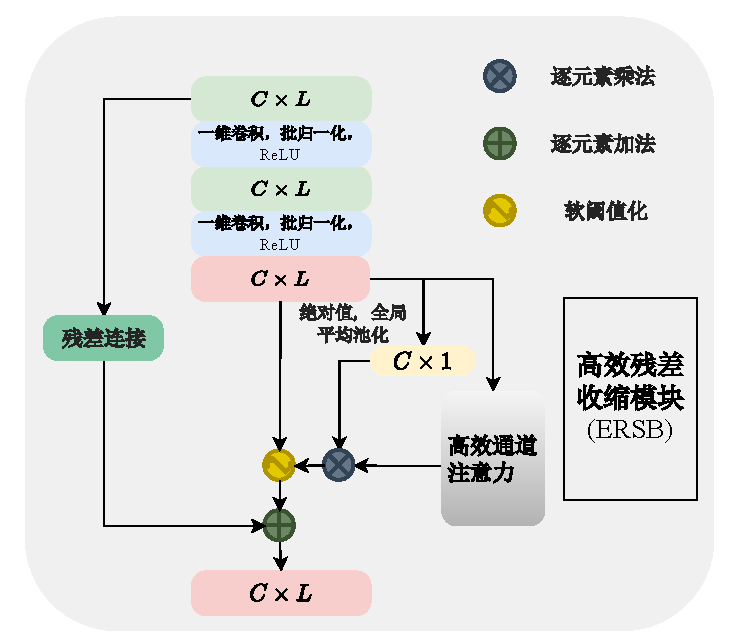
\includegraphics[width=0.6\textwidth]{Image/fem.jpg}
%     \caption{多尺度特征提取模块}
%     \label{fig:fem}
% \end{figure}

% \begin{equation}
%     \begin{aligned}
%             \text{soft-threshold}(x, \lambda) = \begin{cases}
%             x - \lambda, & x > \lambda \\
%             0, & -\lambda \leq x \leq \lambda \\
%             x + \lambda, & x < -\lambda,
%             \end{cases}
%         \end{aligned}
%     \label{equ: soft}
% \end{equation}

% FEM(Feature Extraction Module)的设计旨在从去噪信号中抽取具有多尺度特征的有力表示。采用层次化结构,FEM集成了多个ERSB(Enhanced Residual Shrinkage Block),这种设计灵感源自ResNet架构。ERSB的构建是基于Deep Residual Shrinkage Network中RSB(Residual Shrinkage Block)的思想~\cite{zhao2019deep},但在这里,我们采用了更为高效的ECA模块替代了原始的SE块。如图~\ref{fig:fem} 的右上角所示,ERSB由两个卷积层、身份快捷方式、自适应软阈值操作和ECA模块组成。

% 身份快捷方式的引入不仅使得训练过程中信息流畅通,而且有助于在网络层次中实现梯度的良好传播。自适应软阈值操作,如式~\eqref{equ: soft} 所示,是一种在信号处理领域广泛应用的方法,通过将微小的值置零来实现噪音抑制。ERSB内的自适应软阈值操作与传统的手工设计滤波器不同,它经过训练以自动确定阈值,从而更加适应多样的信号特征。此外,ECA模块通过跨通道整合信息,以更少的参数实现对特征的细致优化,并在泛化性能上胜过SE模块。

% 通过堆叠具有身份快捷方式的多个ERSB,FEM能够分层提取输入信号的多尺度表示,灵活地适应信号的不同频率和结构。这种层次化的特征提取使得FEM能够自适应地将不相关的特征抑制,从而得到更具信息含量的表示。综合来看,身份快捷方式、软阈值操作和ECA模块相互协作,使得FEM在处理输入信号时能够稳健地提取出干净而丰富的多尺度特征。在FEM的详细配置中,我们采用了1D卷积层作为主干,并通过减少输出通道数目来适应信号分类任务,以此平衡了性能和计算复杂性。

\subsection{特征提取模块}\label{sec:background}

\begin{equation}
    \begin{aligned}
            \text{soft-threshold}(x, \lambda) = \begin{cases}
            x - \lambda, & x > \lambda \\
            0, & -\lambda \leq x \leq \lambda \\
            x + \lambda, & x < -\lambda,
            \end{cases}
        \end{aligned}
    \label{equ: soft}
\end{equation}

\begin{figure}
\centering
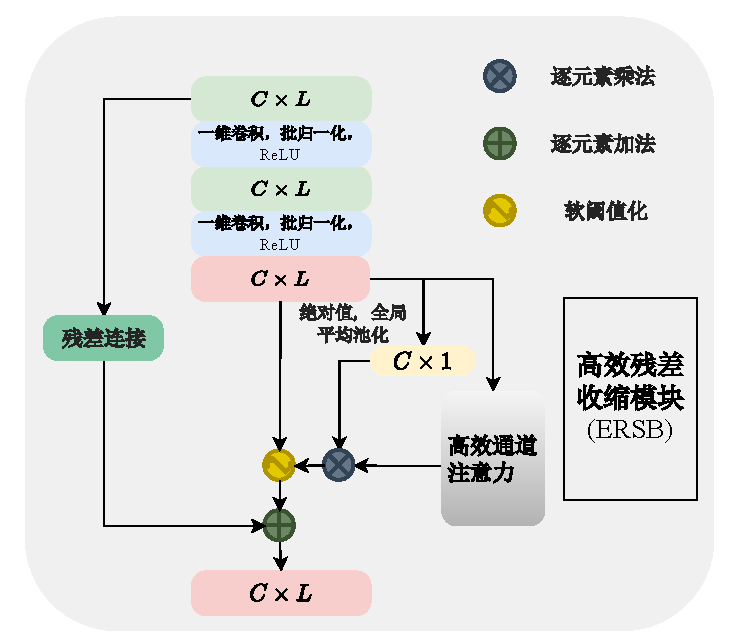
\includegraphics[width=0.8\textwidth]{Image/fem.pdf}
\caption{高效残差收缩模块}
\label{fig:fem}
\end{figure}

FEM(Feature Extraction Module)的设计核心在于从经过降噪处理的信号中有效地提取出具有丰富多尺度特征的表示。本模块采用分层化结构,并集成了多个增强残差收缩块(Enhanced Residual Shrinkage Block, ERSB),这一设计受到了深度残差网络(ResNet)架构的启发。ERSB的构建基于深度残差收缩网络中的残差收缩块(Residual Shrinkage Block, RSB)的概念~\cite{zhao2019deep}。然而,在FEM中,我们采用更高效的ECA模块来替换原始的SE块,以提升网络的性能和效率。

ERSB的设计包括两个关键部分:卷积层和残差连接。卷积层用于捕获信号的局部特征,而残差连接则保证信息的流畅传递,并有助于实现网络层次中梯度的有效传播。此外,我们还引入了自适应软阈值操作,如式~\eqref{equ: soft}所示。这种操作在信号处理领域被广泛应用,用于抑制微小的信号值,从而降低噪音的影响。不同于传统的手动阈值设置,ERSB内的软阈值操作通过训练自动调整,更好地适应多样化的信号特征。

ECA模块在ERSB中发挥着至关重要的作用,它通过跨通道信息整合来精细调节特征,使用较少的参数便达到了优越的泛化能力,超越了SE模块的性能。

FEM通过堆叠多个具有残差连接的ERSB,实现了对输入信号的多层次、多尺度特征提取。这种分层提取机制赋予FEM能够灵活应对信号的各种频率和结构变化。层次化的特征提取方法使得FEM能够有效地抑制不相关特征,提取出更加丰富和信息密集的特征表示。通过这样的结构设计,残差连接、软阈值操作和ECA模块相互协作,确保了FEM在处理输入信号时的稳定性和有效性。

在FEM的具体配置中,我们主要采用1D卷积层作为其主要结构,同时通过调整输出通道数目来适应不同的信号分类任务,实现了性能与计算复杂性之间的平衡。

\begin{figure}
    \centering
    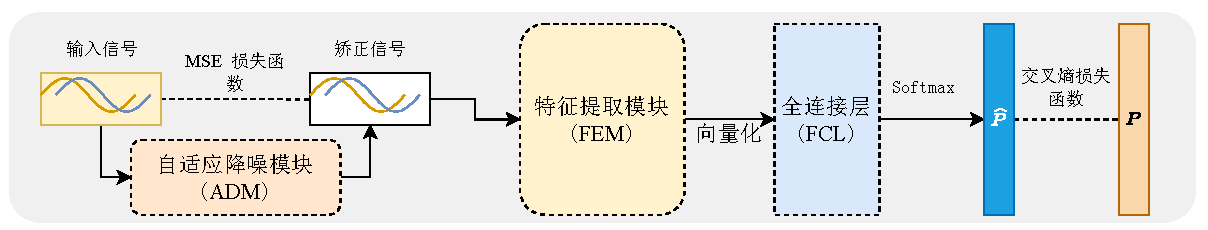
\includegraphics[width=\textwidth]{Image/ad-amr-overview_cn.pdf}
    \caption{整体框架图}
   \label{fig:ad-amr-overview}
\end{figure}

\section{仿真结果}\label{sec:background}
% 数据集 RadioML 2016.10A、 RadioML 2016.10B 和 RadioML 2018.01A
% 以 6:2:2 的比例划分为训练集、验证集和测试集
% 平台:PyTorch 框架,NVIDIA RTX 3090 GPU
% Adam 优化器,学习率为 0.001
% 100 个 epochs, early stopping 技术
% reduce learning rate on plateau 技术用于自适应地调整学习率以搜索最佳参数
% OA、宏平均 F1 分数、Kappa 系数和参数数量作为评价指标
% 比较试验:RadiML 2016.01A 数据集: CNN CLDNN SVM AMC-Net
% 比较试验:RadiML 2016.01B 数据集: CNN CLDNN ResNet AMC-Net
% 比较试验:RadiML 2018.01A 数据集: CNN CLDNN ResNet SENet AWN
% 消融实验: 去掉 ECA 模块 、 去掉 ADM 模块 、 两者都去掉 (同时在上述三个数据集上进行)
% 讨论实验:在现有的模型上添加 ADM 模块,比较结果 (在上述三个数据集上进行)
% 评估指标:OA、宏平均 F1 分数、Kappa 系数和参数数量
\subsection{实验设置}

% #### 数据集及划分
在本研究中,我们旨在评估自适应噪声矫正调制识别网络(ADM)的性能,并与现有的方法进行比较。实验使用了RadioML 2016.10A、RadioML 2016.10B 和 RadioML 2018.01A三个数据集,输入尺寸分别为$2 \times 128$, $2 \times 128$和$2 \times 1024$,它们包含了不同类型的调制信号,适用于评估调制识别算法的性能。数据集被分为训练集、验证集和测试集,按照6:2:2的比例划分。这种划分旨在确保模型在各种条件下都能进行充分的训练和公正的评估。

% #### 实验平台
实验在PyTorch框架下进行,利用NVIDIA RTX 3090 GPU进行计算。PyTorch是当前深度学习研究中广泛使用的框架之一,其灵活性和强大的计算能力为本实验提供了支持。模型的训练采用Adam优化器,初始学习率设置为0.001。所使用的损失函数为交叉熵损失函数,用于衡量模型输出与真实标签之间的差异。交叉熵损失函数的定义如下:

% 交叉熵损失函数
\begin{equation}
\begin{aligned}
\text{CrossEntropy}(y, \hat{y}) = -\sum_{i=1}^{N} y_i \log(\hat{y}_i),
\end{aligned}
\label{equ: crossentropy}
\end{equation}
其中$y$表示真实标签,$\hat{y}$表示模型输出,$N$表示类别数量。

整个训练过程包括100个epochs(训练周期),同时采用了早停止 (early stopping)技术以防止过拟合。早停止是一种在机器学习和深度学习中常用的技术,用于防止模型过拟合同时提高训练效率。这种技术的核心在于监控模型在一个独立的验证集上的性能。在训练过程中,除了在训练集上学习,模型还会在这个验证集上进行评估。验证集通常包含未用于训练的数据,它模拟了模型在未知数据上的表现。早停止的关键在于设置一个“耐心”参数,它定义了在性能没有显著提升的情况下模型继续训练的epoch数量。如果在这些epoch内,模型在验证集上的性能没有提升,或者性能开始下降,训练过程将提前终止。这样做的目的是防止模型过度学习训练数据的特定特征,即防止过拟合,确保模型在未知数据上具有更好的泛化能力。同时,早停止还可以避免在训练深层和复杂网络时的不必要计算,节约计算资源。由于其简单性和有效性,早停止已成为训练深度学习模型时的一个重要工具,尤其在处理大型数据集或构建复杂模型时尤为重要。此外,为了在训练过程中自适应地调整学习率,我们采用了平台期衰减学习率 (reduce learning rate on plateau)技术,平台期衰减学习率 是一种在深度学习训练中常用的学习率调整策略,旨在改善模型在训练过程中的性能和收敛速度。这种方法特别适用于处理模型训练过程中遇到的性能停滞或提升缓慢的情况。当使用这种策略时,学习率的调整基于模型在验证集上的性能指标,如损失或准确率。在连续若干个epoch中,如果模型的性能没有显著提升,即进入了平台),学习率将被自动减少。具体来说,如果模型在设定的epoch数量内未能达到预定的性能改善阈值,学习率会乘以一个事先定义的因子(通常小于1)进行减小。例如,如果当前学习率是0.001,乘以一个因子0.1后,新的学习率将变为0.0001。这种方法的主要优点是在训练过程中提供了一种自适应机制,有助于细致地调整学习率,从而克服学习停滞的挑战。通过降低学习率,模型在参数空间中的搜索步长减小,这有助于更精细地探索,并有可能找到更优的局部最优解。平台期衰减学习率 策略在训练深度网络、尤其是在复杂或高度非凸优化问题中非常有效。它可以避免模型在训练早期由于较大学习率导致的过快收敛到非最优解,同时在训练后期通过更小的学习率细致调整,以提升模型性能。此外,这种策略还有助于提高模型训练的稳定性和可靠性,尤其是在处理大规模数据集时。

% ### 评价指标
我们选用了准确率(Overall Accuracy, OA)、宏平均F1分数、Kappa系数和模型参数数量作为评价指标。OA提供了整体性能的概览,宏平均F1分数评估了模型在不同类别上的均衡性能,Kappa系数则衡量了分类准确性相对于随机分类的改善。参数数量反映了模型的复杂度。
OA定义为:
\begin{equation}
        \begin{aligned}
            \text{OA} = \frac{\sum_{i=1}^{M}TP_i}{\sum_{i=1}^{M}TP_i + \sum_{i=1}^{M}FP_i},
        \end{aligned}
    \label{equ: oa}
\end{equation}
F1分数定义为:
\begin{equation}
    \begin{aligned}
        \text{F1-score} = \frac{2\sum_{i=1}^{M}TP_i}{2\sum_{i=1}^{M}TP_i + \sum_{i=1}^{M}FP_i + \sum_{i=1}^{M}FN_i},
    \end{aligned}
    \label{equ: f1}
\end{equation}
Kappa系数定义为:
\begin{equation}
    \begin{aligned}
        \text{Kappa} = \frac{\text{OA} - \mathbb{P}(\text{Chance})}{1 - \mathbb{P}(\text{Chance})},
    \end{aligned}
    \label{equ: kappa}
\end{equation}
其中$TP_i$是正确分类为第$i$种调制的样本数量,$FP_i$是错误分类为第$i$种调制的样本数量,$\mathbb{P}(\text{Chance})$表示随机分类的概率。

% ### 比较试验
为了全面评估ADM的性能,我们在三个数据集上进行了一系列比较试验,具体的实验内容如表~\ref{tab:experiment_summary}所示。

\begin{table}[htpb]
    \centering
    \caption{实验概览}
    \resizebox{\textwidth}{!}{%
    \label{tab:experiment_summary}
    \begin{tabular}{cm{0.25\textwidth}m{0.25\textwidth}m{0.5\textwidth}}
    \hline
    \textbf{实验类型} & \textbf{RadiML 2016.10A} & \textbf{RadiML 2016.10B} & \textbf{RadiML 2018.01A} \\ \hline
    基准比较 & CNN, CLDNN, SVM & ResNet, AMC-Net & CNN, CLDNN, ResNet, SENet, AWN \\ \hline
    消融实验 & \multicolumn{3}{c}{1. 去掉ECA模块, 2. 去掉ADM模块, 3. 将前两者都去掉} \\ \hline
    讨论实验 & \multicolumn{3}{c}{在现有模型(CNN, CLDNN, ResNet, SENet, AWN) 上添加ADM模块} \\ \hline
    \end{tabular}
    }
\end{table}

在本研究中,我们精心设计了一系列实验,以全面评估自适应噪声矫正调制识别网络(ADM)的性能,并将其与当前的主流方法进行比较。实验设计的理念是基于不同数据集的特性来选择最合适的比较模型,以确保评估的全面性和公正性。

首先,我们选择了RadioML 2016.10A数据集进行初步的性能比较。这个数据集相对较小,因此特别适合用来评估简单模型的性能,并与传统的算法,如支持向量机(SVM),进行比较。由于数据集的规模较小,它提供了一个理想的环境,用于快速验证模型的基本性能和稳定性。在这个阶段,我们主要关注模型在基本调制识别任务上的能力,以及它与传统机器学习方法在处理这类问题时的相对优势。

随后,我们转向RadioML 2016.10B数据集,该数据集在样本维度上与2016.10A一致,但总体规模更大。较大的数据集规模使得它更适合用来评估近几年深度学习模型的性能。在这个阶段,我们将AD-AMR Net与如残差网络(ResNet),AMC-Net等近年来流行的深度学习模型进行对比。通过这样的比较,我们能够更好地理解ADM在处理相对复杂的数据集时的表现,以及其在现代深度学习框架中的竞争力。

最后,我们使用RadioML 2018.01A数据集,这是一个在样本维度和数据集本身都较大的数据集。这个数据集适合用来与当前主流的深度学习模型进行比较,如SENet和自适应小波网络(AWN)。这个阶段的实验不仅能够展示AD-AMR Net在处理大规模、高维度数据时的能力,还能揭示其在最先进的模型面前的性能和适应性。

在消融实验中,我们的主要目的是证明所提出模块的有效性。通过分别去掉ECA模块、ADM模块以及两者都去掉的设置,我们可以详细分析每个组件对整体性能的贡献,以及它们之间的相互作用。这种方法能够清晰地展示每个模块的重要性,以及它们如何共同作用以提高模型的整体性能。消融实验的具体设置如下:
\begin{enumerate}
    \item AD-AMR Net:完整的提出模型。

    \item AD-AMR~-~1:去除ADM的提出模型。

    \item AD-AMR~-~2:去除FEM中ERSB的提出模型。

    \item AD-AMR~-~3:去除ADM和FEM中ERSB的提出模型。
\end{enumerate}

此外,在讨论实验中,我们探讨了ADM模块的“即插即用”能力,即评估将ADM模块加入到现有模型中时的效果。这项工作不仅验证了ADM模块的通用性,还展示了其在不同架构中的适应性和效果。通过这些实验,我们能够全面评价ADM模块在不同设置和环境下的实际应用价值。讨论实验的具体设置如下:
\begin{enumerate}
    \item ADM-CNN:带有ADM的CNN。
    \item ADM-CLDNN:带有ADM的CLDNN。
    \item ADM-AWN:带有ADM的AWN。
\end{enumerate}

综上所述,通过这些精心设计的实验,我们不仅能够全面评估ADM在不同数据集和环境中的性能,还能深入理解其与现有方法的比较情况,以及单独模块对整体性能的影响。这些实验结果将为调制识别领域的研究提供宝贵的见解,推动相关技术的进一步发展。

% 我们在PyTorch中实现了AD-AMR Net,并在NVIDIA RTX 3090 GPU上从头开始进行了训练。网络经过了100个epochs的训练,使用了Adam优化器,学习率为0.001。我们采用了\textit{early stopping}技术,即如果验证损失在连续10次迭代后不再减小,则停止训练,以防止过拟合并提高训练效率。

% 为了自适应地调整学习率以搜索最佳参数,我们还采用了\textit{reduce learning rate on plateau}技术,即当损失指标停止改善时减小学习率。这种自适应调整有助于更有效地在参数空间中导航。

% 对于训练和评估,我们选择了RadioML 2018.01A数据集~\cite{o2018over}。该数据集提供了一个全面的场景集,可以在不同的无线信道效应下对AD-AMR Net进行深入检查,包括多径衰落、采样率偏移、加性白噪声(AWGN)和中心频率偏移等。

% 在整个训练和评估阶段,我们进行了数值分析,以评估所提出方案的性能。通过在不同无线信道条件下进行测试,验证了模型的鲁棒性和适应性。这次全面的评估旨在展示AD-AMR Net在处理不同信道干扰引起的真实世界挑战方面的有效性。

% \subsection{性能指标}

% 我们使用整体准确度(Overall Accuracy, OA)、宏平均F1分数、Kappa系数和参数数量作为评价指标,其中
% OA定义为:
% \begin{equation}
%         \begin{aligned}
%             \text{OA} = \frac{\sum_{i=1}^{M}TP_i}{\sum_{i=1}^{M}TP_i + \sum_{i=1}^{M}FP_i},
%         \end{aligned}
%     \label{equ: oa}
% \end{equation}
% F1分数定义为:
% \begin{equation}
%     \begin{aligned}
%         \text{F1-score} = \frac{2\sum_{i=1}^{M}TP_i}{2\sum_{i=1}^{M}TP_i + \sum_{i=1}^{M}FP_i + \sum_{i=1}^{M}FN_i},
%     \end{aligned}
%     \label{equ: f1}
% \end{equation}
% Kappa系数定义为:
% \begin{equation}
%     \begin{aligned}
%         \text{Kappa} = \frac{\text{OA} - \mathbb{P}(\text{Chance})}{1 - \mathbb{P}(\text{Chance})},
%     \end{aligned}
%     \label{equ: kappa}
% \end{equation}
% 其中$TP_i$是正确分类为第$i$种调制的样本数量,$FP_i$是错误分类为第$i$种调制的样本数量,$\mathbb{P}(\text{Chance})$表示随机分类的概率。

% \dots

% \subsection{基准比较}
% 为了评估,将使用以下方法与所提出的方案进行比较作为基准:
% \begin{enumerate}
%     \item \textit{CNN}~\cite{o2016convolutional}:CNN是一种基本的卷积神经网络,使用卷积层从复杂的信号输入中提取特征并对调制类型进行分类。
%     \item \textit{CLDNN}~\cite{sainath2015convolutional}:CLDNN结合了CNN和RNN结构,使用四个卷积层、一个LSTM层和两个全连接层。
%     \item \textit{ResNet}~\cite{liu2017deep}:ResNet是一种深度卷积网络架构,通过跳跃连接来减少深度神经网络中的梯度消失问题。
%     \item \textit{SENet}~\cite{zhang2023frequency}:SENet将挤压和激励(SE)块与ResNet集成,以提高特征学习效果。
%     \item \textit{AWN}~\cite{zhang2023towards}:自适应小波网络(AWN)结合自适应小波分解和通道注意机制,将复杂信号分解并学习用于分类的优化频率特征。
% \end{enumerate}

\subsection{实验结果}

\begin{table}[h]
    \centering
    \caption{不同模型在RadioML数据集上的性能比较}
    \label{tab:model_comparison}
    \resizebox{\textwidth}{!}{%
    \begin{tabular}{ccccccc}
    \hline
    \textbf{数据集}               & \textbf{模型}      & \textbf{OA} & \textbf{F1-score} & \textbf{Kappa} & \textbf{0-10dB准确率} & \textbf{参数量} \\ \hline
    \multirow{2}{*}{RadioML 2016.10A} & CLDNN     & 0.5621 & 0.5721 & 0.5184 & 0.8219 & \textbf{0.09M} \\ \cline{2-7} 
                                  & PROPOSED      & \textbf{0.6155} & \textbf{0.6412} & \textbf{0.5771} & \textbf{0.8988} & 0.21M \\ \hline
    \multirow{2}{*}{RadioML 2016.10B} & CLDNN     & 0.5846 & 0.5796 & 0.5385 & 0.8416 & \textbf{0.09M} \\ \cline{2-7} 
                                  & PROPOSED      & \textbf{0.6485} & \textbf{0.6500} & \textbf{0.6094} & \textbf{0.9292} & \textbf{0.21M} \\ \hline
    \multirow{6}{*}{RadioML 2018.01A} & CNN       & 0.5820 & 0.5854 & 0.5639 & 0.7229 & 0.48M \\ \cline{2-7} 
                                  & CLDNN         & 0.5772 & 0.5755 & 0.5588 & 0.7213 & 1.32M \\ \cline{2-7} 
                                  & ResNet        & 0.6211 & 0.6226 & 0.6047 & 0.8072 & 7.23M \\ \cline{2-7} 
                                  & SENet         & 0.6327 & 0.6391 & 0.6168 & 0.8287 & 7.39M \\ \cline{2-7} 
                                  & AWN           & 0.6262 & 0.6262 & 0.6099 & 0.8036 & 0.38M \\ \cline{2-7} 
                                  & PROPOSED      & \textbf{0.6460} & \textbf{0.6480} & \textbf{0.6306}  & \textbf{0.8480} & \textbf{0.25M} \\ \hline
    \end{tabular}
    }
\end{table}



\begin{table}[ht]
    \caption{消融实验结果}
    \begin{center} 
        \resizebox{0.8\textwidth}{!} & -2.11\% & \textbf{-2.34\%} & \textbf{-4.62\%} & -0.11M \\
                \hline
                AD-AMR~- 2 & 0.6241 & 0.6254 & 0.6078 & 0.8097 & 0.25M \\
                $\Delta$ & -2.23\% & \textbf{-2.26\%} & -2.28\% & -3.83\% & -0.00M \\
                \hline
                AD-AMR~- 3 & 0.6067 & 0.6086 & 0.5896 & 0.7794 & \textbf{0.14M} \\
                $\Delta$ & -3.93\% & -3.94\% & -4.10\% & -6.86\% &-0.11M \\
                \hline
                \textbf{AD-AMR Net} & \textbf{0.6460} & \textbf{0.6480} & \textbf{0.6306}  & \textbf{0.8480} & 0.25M \\
                \hline
            \end{tabular}
            }
    \end{center}
~\label{tab: ablation}
\end{table}

\begin{figure}
    \centering
    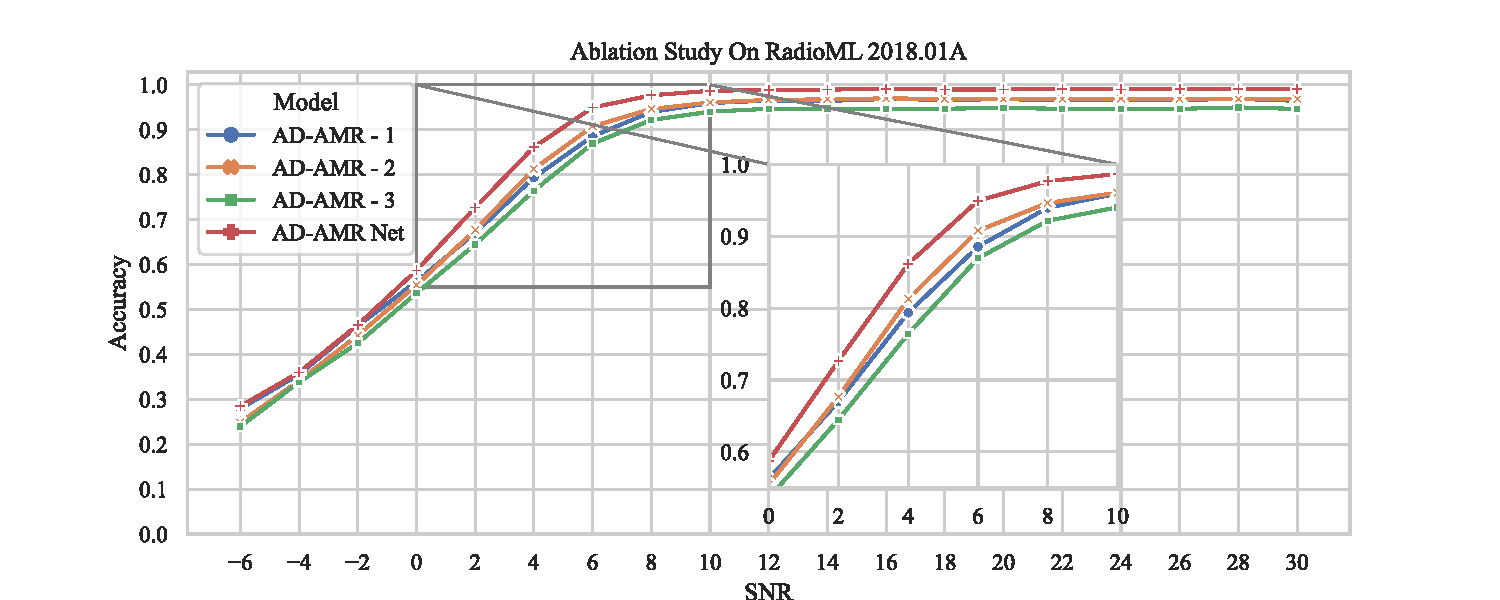
\includegraphics[width=\textwidth]{Image/ablation_res.pdf}
    \caption{消融实验结果}
    \label{fig: ablation_res}
\end{figure}

\begin{table}[ht]
    \caption{讨论结果}
    \begin{center} 
        \resizebox{0.8\textwidth}{!} & +3.29\% & \textbf{+3.51\%}  & \textbf{+6.67\%} & +0.11M \\
                \hline
                ADM-CLDNN & 0.5994 & 0.6126 & 0.5820 & 0.7638 & 1.43M \\
                $\Delta$ & +2.22\% & \textbf{+3.71\%} & +2.32\% & +4.25\% & +0.11M \\
                \hline
                ADM-AWN & 0.6300 & 0.6300 & 0.6139 & 0.8271 & 0.49M \\
                $\Delta$ & +0.38\% & +0.38\% & +0.4\% & +2.35\% & +0.11M \\
                \hline
            \end{tabular}
        }
    \end{center}
~\label{tab: discussion}
\end{table}

\begin{figure}
    \centering
    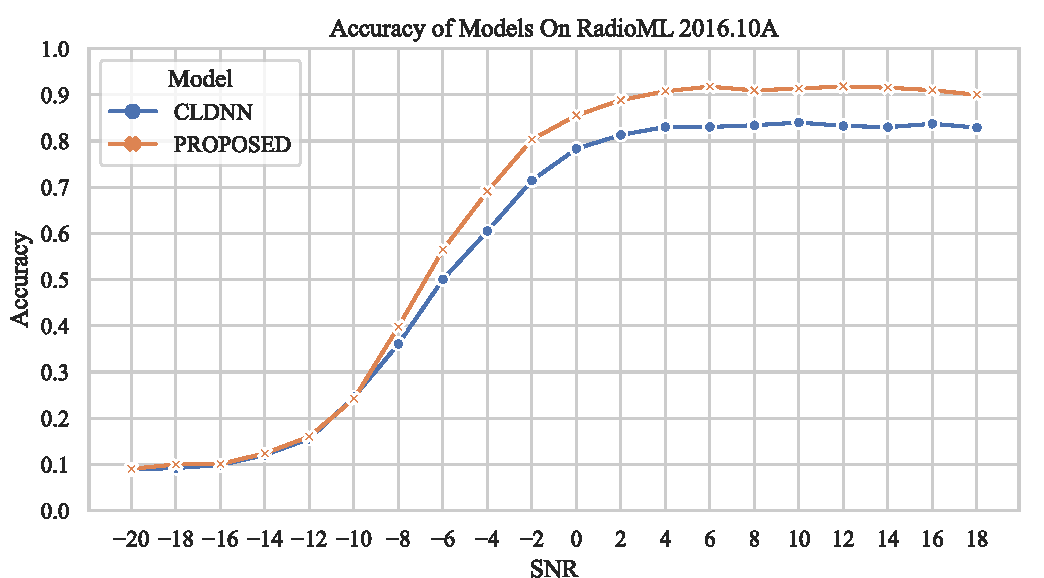
\includegraphics[width=\textwidth]{Image/16a_acc.pdf}
    \caption{不同模型在不同信噪比下的性能比较 (RadioML 2016.10A数据集)}
    \label{fig:2016A_res}
\end{figure}

\begin{figure}[ht]
    \centering
    \begin{subfigure}[b]{0.45\textwidth}
      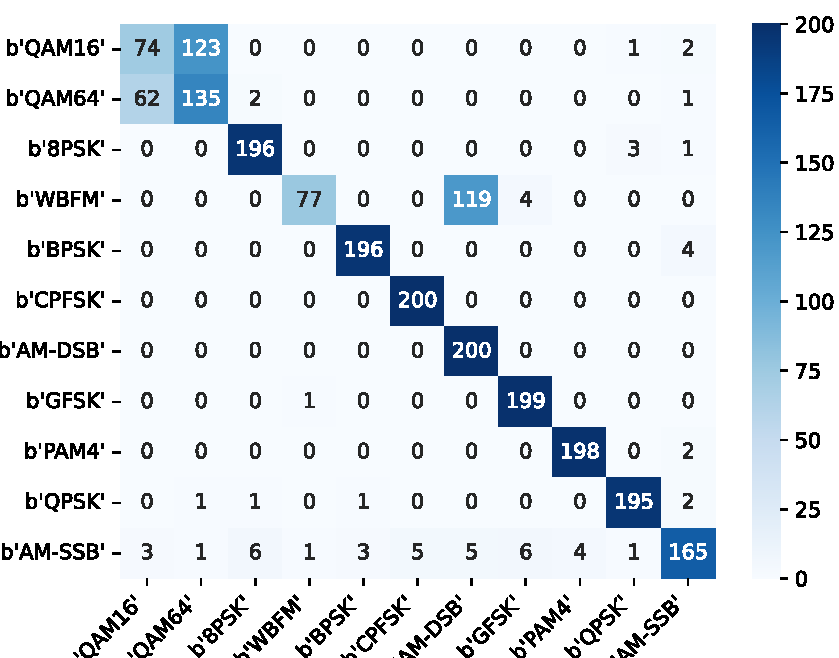
\includegraphics[width=\textwidth]{Image/cldnn_16a.pdf}
      \label{fig:image1}
    \end{subfigure}
    \hfill
    \begin{subfigure}[b]{0.45\textwidth}
      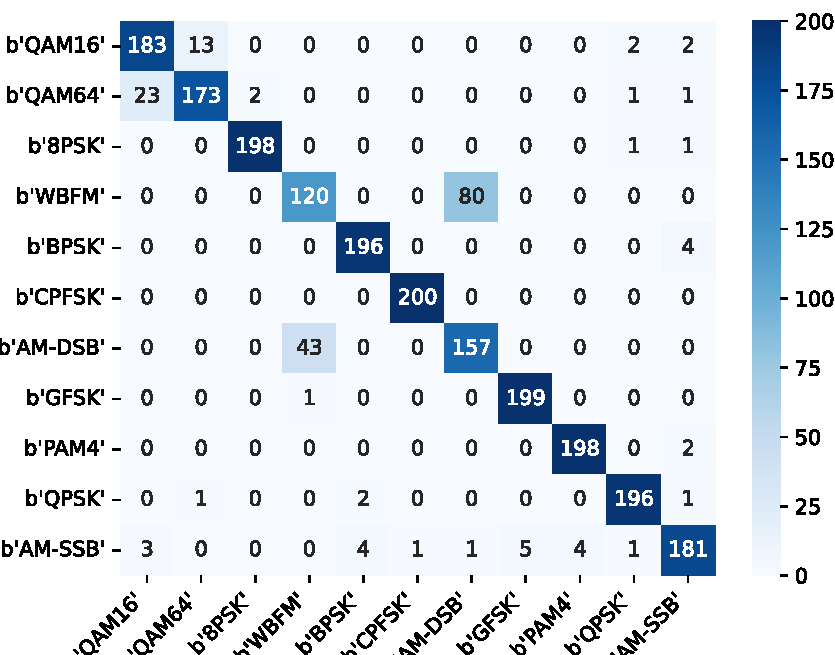
\includegraphics[width=\textwidth]{Image/proposed_16a.pdf}
      \label{fig:image2}
    \end{subfigure}
    \caption{8dB 混淆矩阵 (RadioML 2016.10A数据集, 左:CLDNN, 右:AD-AMR Net)}
    \label{fig:16a_matrix}
  \end{figure}
  
\begin{figure}
    \centering
    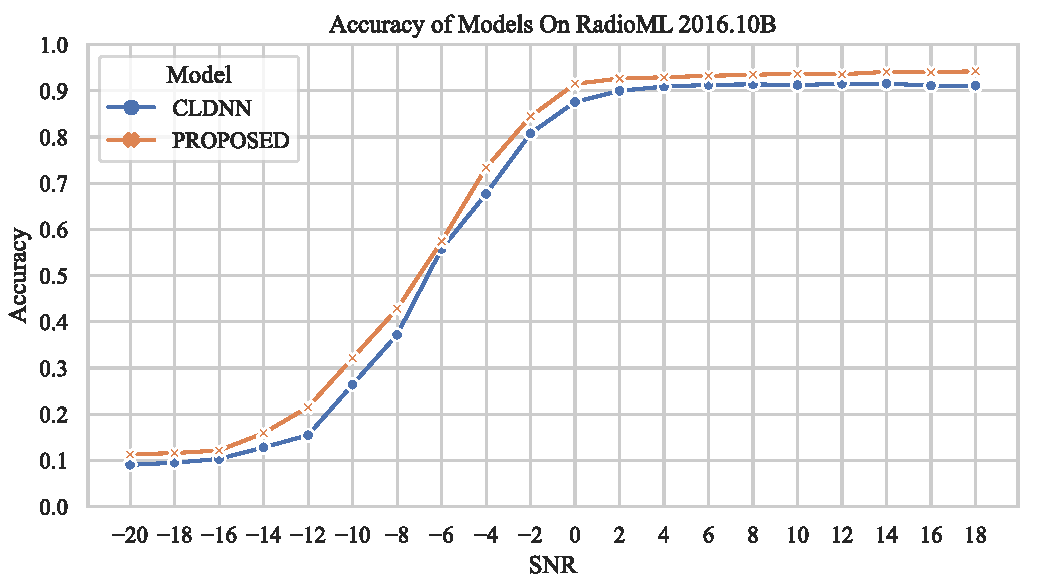
\includegraphics[width=\textwidth]{Image/16b_acc.pdf}
    \caption{不同模型在不同信噪比下的性能比较 (RadioML 2016.10B数据集)}
    \label{fig:2016B_res}
\end{figure}

\begin{figure}[ht]
    \centering
    \begin{subfigure}[b]{0.45\textwidth}
      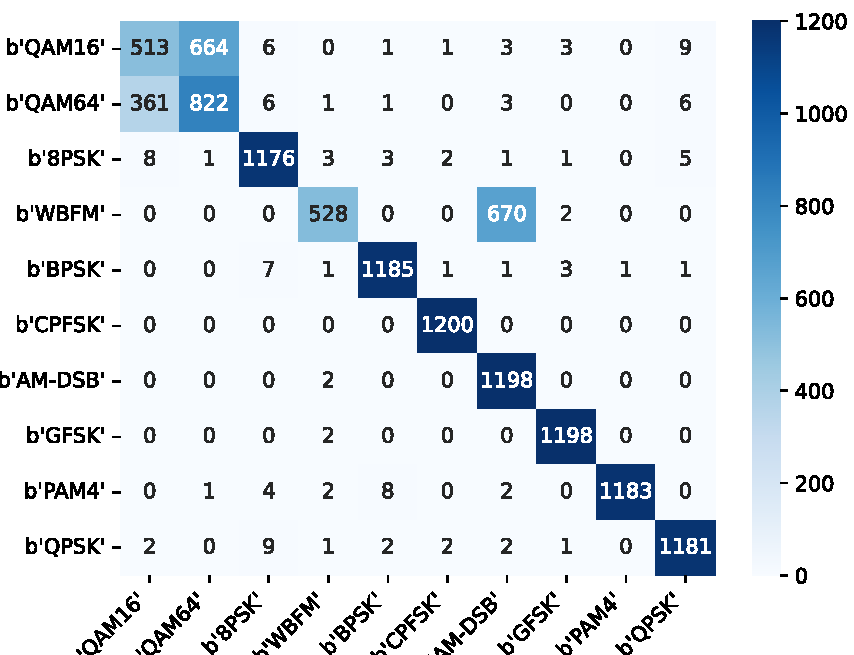
\includegraphics[width=\textwidth]{Image/cldnn_16b.pdf}
      \label{fig:image1}
    \end{subfigure}
    \hfill
    \begin{subfigure}[b]{0.45\textwidth}
      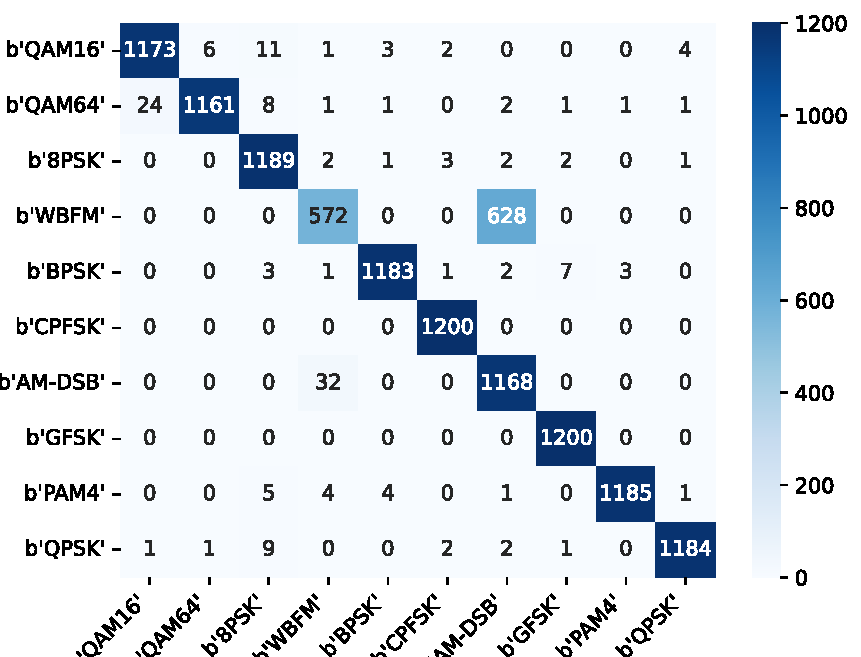
\includegraphics[width=\textwidth]{Image/proposed_16b.pdf}
      \label{fig:image2}
    \end{subfigure}
    \caption{8dB 混淆矩阵 (RadioML 2016.10B数据集, 左:CLDNN, 右:AD-AMR Net)}
    \label{fig:16a_matrix}
  \end{figure}

  \begin{figure}
    \centering
    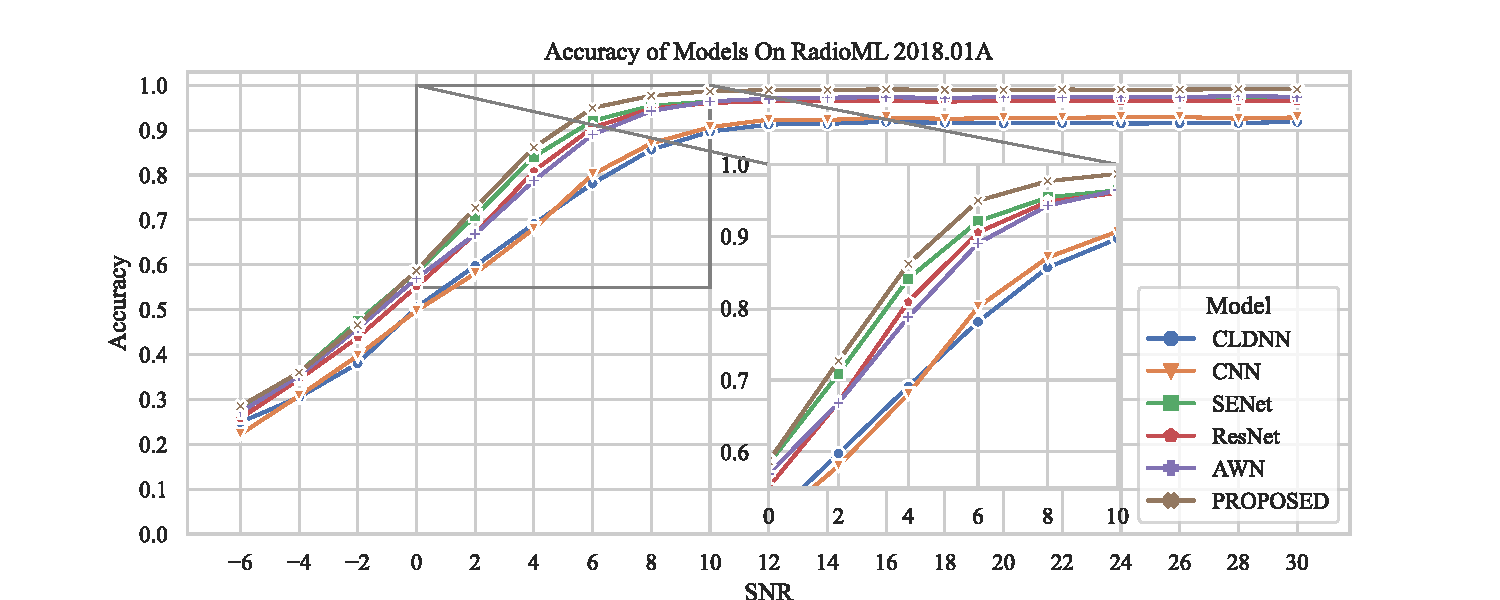
\includegraphics[width=\textwidth]{Image/model_res.pdf}
    \caption{不同模型在不同信噪比下的性能比较 (RadioML 2018.01A数据集)}
    \label{fig:model_acc}
\end{figure}


\begin{figure}[ht]
    \centering
    \begin{subfigure}[b]{0.45\textwidth}
      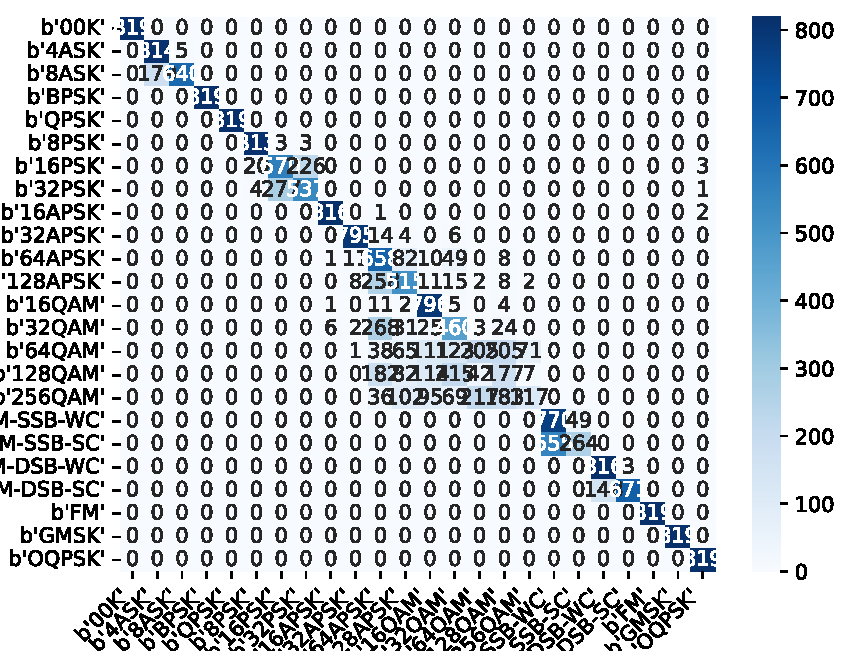
\includegraphics[width=\textwidth]{Image/cldnn_18a.pdf}
      \label{fig:image1}
    \end{subfigure}
    \hfill
    \begin{subfigure}[b]{0.45\textwidth}
      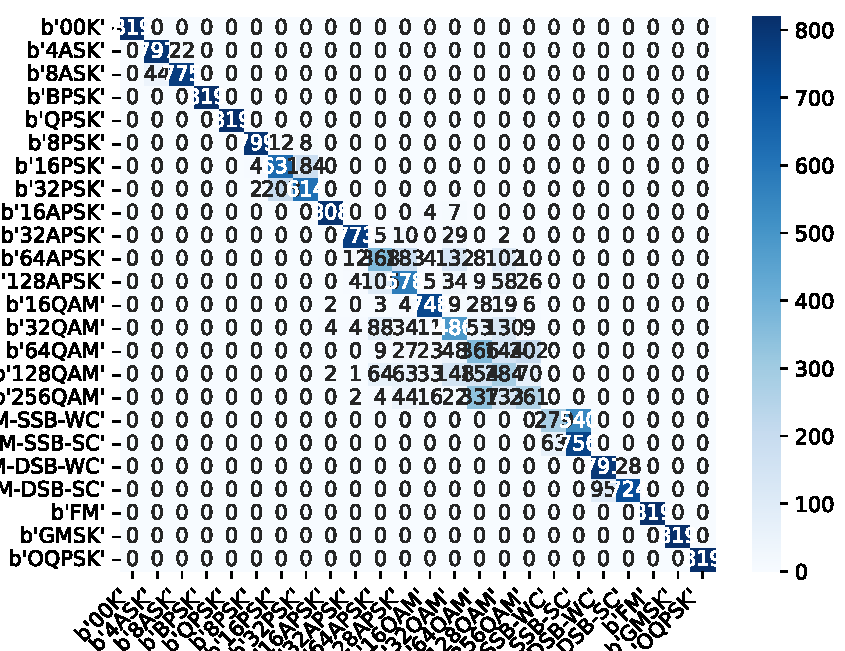
\includegraphics[width=\textwidth]{Image/cnn_18a.pdf}
      \label{fig:image2}
    \end{subfigure}
    \hfill
    \begin{subfigure}[b]{0.45\textwidth}
        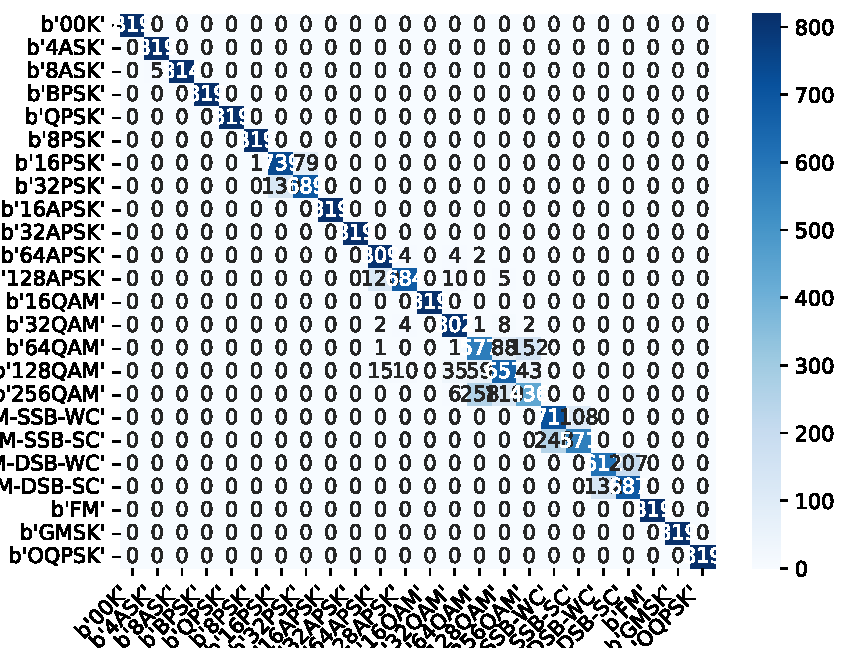
\includegraphics[width=\textwidth]{Image/resnet_18a.pdf}
        \label{fig:image2}
      \end{subfigure}
      \hfill
      \begin{subfigure}[b]{0.45\textwidth}
        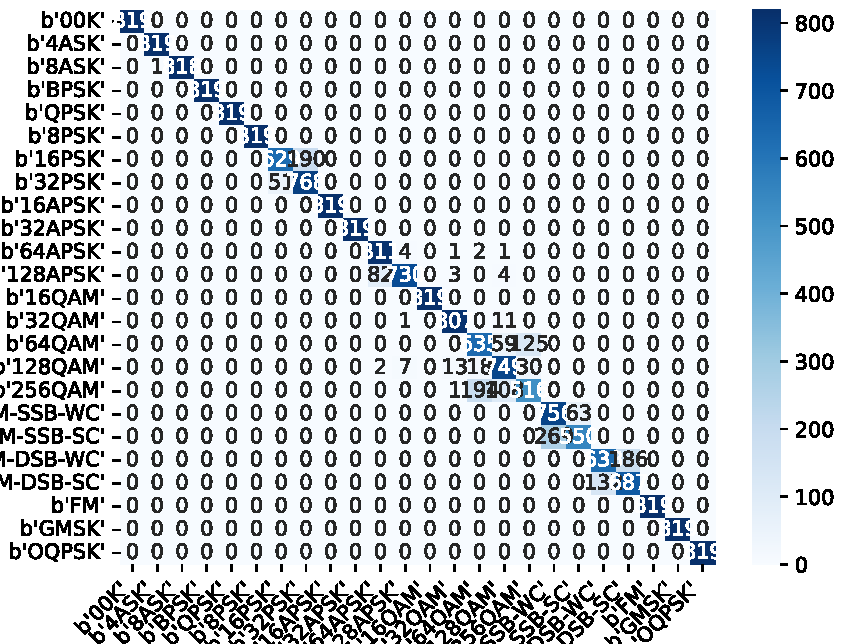
\includegraphics[width=\textwidth]{Image/senet_18a.pdf}
        \label{fig:image2}
      \end{subfigure}
      \hfill
      \begin{subfigure}[b]{0.45\textwidth}
        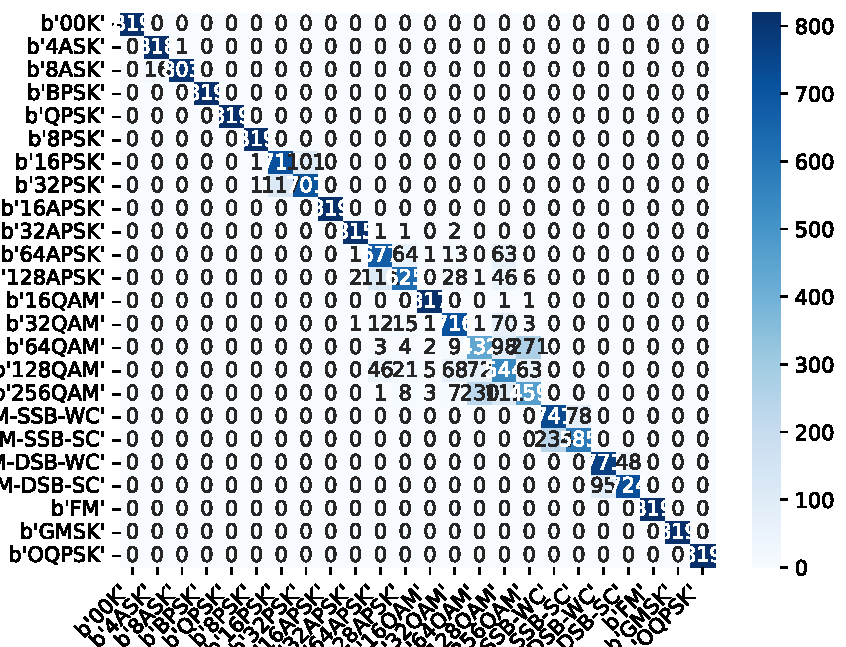
\includegraphics[width=\textwidth]{Image/awn_18a.pdf}
        \label{fig:image2}
      \end{subfigure}
      \hfill
        \begin{subfigure}[b]{0.45\textwidth}
            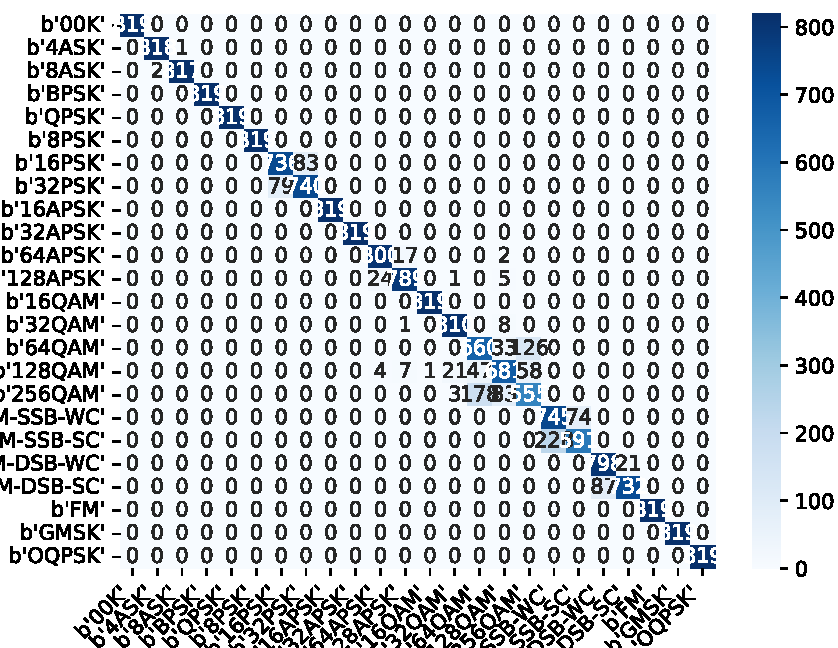
\includegraphics[width=\textwidth]{Image/proposed_18a.pdf}
            \label{fig:image2}
            \end{subfigure}
    \caption{6dB 混淆矩阵 (RadioML 2018.01A数据集, 从左到右,从上到下:CLDNN, CNN, ResNet, SENet, AWN, AD-AMR Net)}
    \label{fig:16a_matrix}
  \end{figure}

在对RadioML 2018.01A数据集进行的实验中,AD-AMR Net模型表现出了明显的性能优势。图~\ref{fig:model_acc}和表~\ref{tab:model_comparison}详细展示了各种模型的性能对比。AD-AMR Net不仅在高信噪比环境中表现优异,更在低信噪比(SNR)环境中展现出了卓越的鲁棒性,这在调制信号识别领域尤为重要。在0~-~10 dB SNR范围内,AD-AMR Net的准确率高达84.8\%,远超其他模型的80~-~82\%。这一显著的性能提升在参数数量显著减少的情况下实现,凸显了模型在效率和性能之间取得了良好的平衡。

我们进一步通过消融实验(表~\ref{tab: ablation})探究了AD-AMR Net内部各组件的作用。去除ADM模块(AD-AMR~-~1)的实验结果显示,性能在所有指标上都有显著下降,特别是在低信噪比条件下,这强调了ADM在提高模型识别能力方面的关键作用。另一方面,仅去除FEM中的ERSB(AD-AMR~-~2)虽然对性能有一定影响,但下降幅度较小。若同时去除这两个核心组件(AD-AMR~-~3),则会导致性能的显著下降,特别是在复杂的信号场景中。这些结果不仅证实了ADM和FEM在提升低信噪比环境下准确性方面的重要性,也突出了它们在维持模型整体性能中的协同作用。

为进一步验证ADM的即插即用特性,我们将ADM应用于其他主流模型,并观察其对性能的影响。如表~\ref{tab: discussion}所示,实验结果表明,不论是在高信噪比还是低信噪比环境下,ADM的加入都能显著提升模型的准确度。这一发现不仅证实了ADM在多种不同环境下的适用性,也展示了它作为一个独立模块对于提高现有模型性能的潜力。

综上所述,通过对AD-AMR Net的全面评估,我们不仅证实了其在多种信噪比环境下的优异性能,也展示了其内部组件的重要性。这些发现为未来调制信号识别模型的设计提供了宝贵的参考,并为进一步提升这类模型的性能和适用性奠定了基础。

\section{本章总结}\label{sec:background}
本章节详细介绍了我们针对自适应噪声矫正调制识别网络(ADM)的一系列实验设计,目的是全面评估ADM在调制识别任务中的性能,并与当前的主流方法进行比较。通过对RadioML 2016.10A、RadioML 2016.10B 和 RadioML 2018.01A三个数据集的深入研究,我们能够在不同规模和复杂性的数据集上测试ADM的有效性。

在实验设计中,我们首先使用较小的RadioML 2016.10A数据集来进行基本的性能比较,特别是与传统的机器学习算法如支持向量机(SVM)进行对比,以验证ADM在基础调制识别任务上的能力。随后,针对更大规模的RadioML 2016.10B数据集,我们将ADM与近年来的深度学习模型如CNN、CLDNN和ResNet进行比较,以评估ADM在处理较复杂数据时的性能。最后,在规模和维度上更大的RadioML 2018.01A数据集上,我们将ADM与当前的主流模型如SENet和AWN进行了比较,进一步验证了ADM在最先进的模型面前的竞争力。

此外,通过一系列消融实验,我们深入分析了ADM中各个组件的作用,特别是ECA模块和ADM模块对整体性能的贡献。这些实验不仅显示了每个单独组件的重要性,也揭示了它们在提升整体模型性能方面的协同作用。在讨论实验中,我们探索了ADM模块的“即插即用”能力,即将其加入到现有模型中的效果,从而展示了ADM模块的通用性和适应性。

综上所述,本章节的实验设计和结果分析为调制识别领域提供了重要的见解,证明了ADM在提升调制识别性能方面的有效性。ADM的成功实施不仅展示了深度学习在解决实际通信问题中的潜力,也为未来在该领域的研究提供了有价值的参考。通过这些实验,我们能够更好地理解深度学习技术在处理复杂信号数据中的应用,以及如何通过创新的模块设计来提升模型性能和效率。
